\chapter{Allgemeine Grundlagen}\label{chapter: Allgemeine Grundlagen}
\thispagestyle{empty}
\section{Bewertung verwendeter Erzeugungsanlagen}
Dieser Abschnitt stellt potentielle Technologien vor, die in einem solarthermisch gestützten Wärmeversorgungssystem zum Einsatz kommen können. Da das Ziel dieser Arbeit die Bewertung eines solchen Systems ist, wird an dieser Stelle auf eine ausführliche Beschreibung jeder einzelnen Technologie verzichtet. Die entsprechenden Unterabschnitte stellen die technologie-spezifischen Besonderheiten kurz dar und zeigen eine mögliche technische Bewertung in Form von Wirkungsgraden.
\subsection{Kraft-Wärme-Kopplung}
Unter \acf{KWK} ist die gekoppelte Erzeugung elektrischer Energie und Wärme zu verstehen. Somit stellt die \ac{KWK} eine Möglichkeit zur Sektorkopplung zwischen elektrischer Energie und Wärme dar. Im Gegensatz zu konventionellen Kraftwerken wird in Heizkraftwerken die Abwärme auf einem höheren, zu Heizzwecken nutzbaren, Temperaturniveau abgegeben. Insgesamt steigt dadurch die Brennstoffausnutzung des Kraftwerks. Um \ac{KWK}-Anlagen bewerten zu können werden folgende Kennzahlen verwendet \cite{VDI4608}:
	\begin{enumerate}
		\item Die \textbf{Heizausbeute} $\alpha$ setzt den abgegebenen Heizwärmestrom $\dot{Q}_\text{H,KWK}$ mit der zugeführten Energie ausgedrückt durch den Brennstoffmassenstrom $\dot{m}_\text{Br}$ und den Heizwert $H_\text{i}$ ins Verhältnis
		\begin{equation}\label{equation: Heizausbeute}
			\alpha = \dfrac{|\dot{Q}_\text{H,KWK}|}{\dot{m}_\text{Br}H_\text{i}}
		\end{equation}	
		
		\item Die \textbf{Stromausbeute} $\beta$ vergleicht entsprechend die abgegebene elektrische Leistung $P_\text{KWK}$ mit der zugeführten Energie
		\begin{equation}\label{equation: Stromausbeute}
			\beta = \dfrac{|P_\text{KWK}|}{\dot{m}_\text{Br}H_\text{i}}
		\end{equation}
		
		\item Der \textbf{Gesamtnutzungsfaktor} $\omega$ einer \ac{KWK}-Anlage ergibt sich nun aus der Summe der Strom- und Heizausbeute
		\begin{equation}\label{equation: Gesamtnutzungsfaktor}
			\omega = \alpha + \beta = \dfrac{|\dot{Q}_\text{H,KWK}| + |P_\text{KWK}|}{\dot{m}_\text{Br}H_\text{i}}
		\end{equation}
	\end{enumerate}
Das Betriebsverhalten von \ac{KWK}-Anlagen kann über das sogenannte PQ-Diagramm beschrieben werden, welches sich je nach verwendeter Technologie unterscheidet. Abbildung \ref{fig: PQ-Diagramm} zeigt beispielhaft die PQ-Diagramme drei unterschiedlicher Technologien. Die Schnittpunkte an der Ordinate stellen die maximal und minimal mögliche elektrische Leistung ohne Wärmeauskopplung dar. Bei der Entnahmeturbine (CCET) sorgt eine Erhöhung der ausgekoppelten Wärme zu einer Reduzierung der elektrischen Leistung, da weniger Dampf in den Endstufen der Turbine zur Verfügung steht. Dies ist beim motorischen Blockheizkraftwerk (mCHP) nicht der Fall. Bei Gegendruckturbinen (BPT) ist die elektrische Leistung fest mit der Wärmeauskopplung verbunden. Für jeden Lastpunkt kann nur eine Kombination aus elektrischer Leistung und Wärmestrom abgegeben werden. Das Gegendruckkraftwerk verfügt also über einen einzigen Freiheitsgrad. Das PQ-Diagramm reduziert sich zu einer einfachen Linie.
	\begin{figure}[htbp]
		\centering
		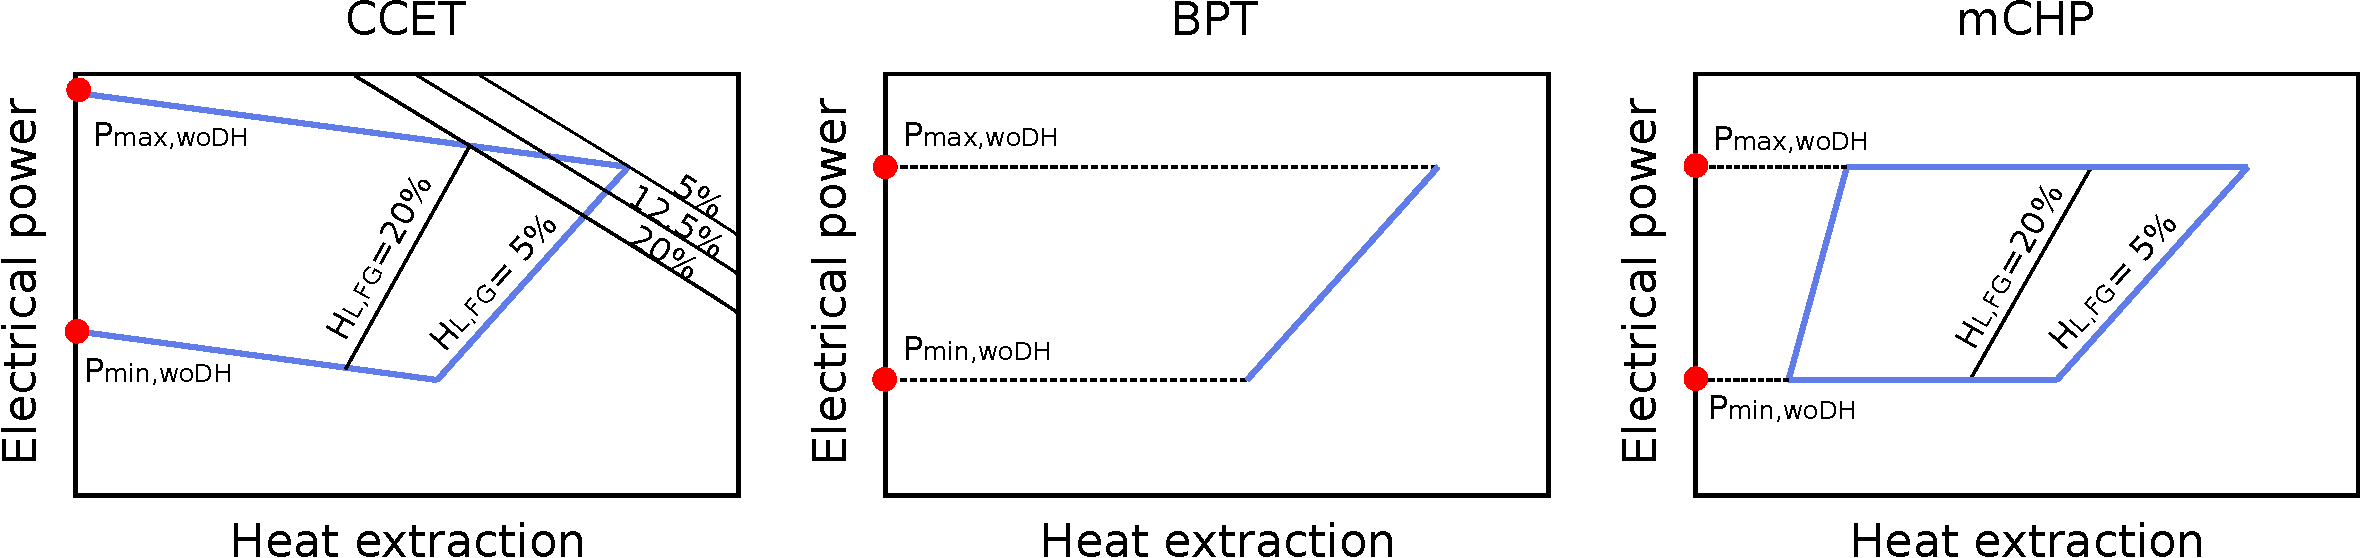
\includegraphics[width=1\linewidth]{GenericCHP.pdf}
		\captionof{figure}[Schematische Darstellung der PQ-Diagramme verschiedener KWK-Anlagen]{Schematische Darstellung der PQ-Diagramme verschiedener KWK-Anlagen. Von links: Ein \ac{GuD} mit Entnahmeschaltung (combined cycle extraction turbines - CCET), einer Gegendruckturbine (back pressure turbine - BPT) und eines motorischen Blockheizkraftwerks (motoric combined heat and power - mCHP) übernommen aus \cite{oemof2019}}
		\label{fig: PQ-Diagramm}
	\end{figure}

\subsection{Thermische Energiespeicher}

\ac{TES} bieten die Möglichkeit der zeitlichen Entkopplung der Wärmebereitstellung und des Bedarfs. Sie werden in drei verschiedenen Arten ausgeführt. Dies sind sensible Wärmespeicher, die eine fühlbare Änderung der Temperatur zur Wärmespeicherung nutzen, latent Wärmespeicher, bei denen zusätzlich die Energie des Phasenwechsels genutzt wird und schließlich thermochemische Wärmespeicher, die chemische Reaktionen zur Wärmespeicherung verwenden. Am besten erforscht und am kostengünstigsten sind die sensiblen Wärmespeicher, weshalb diese Speicher in der Wärmeversorgung vorzugsweise eingesetzt werden. \cite{Sterner2017}

Es gibt zwei mögliche Einsatzzwecke:
	\begin{description}[leftmargin=!,labelwidth=\widthof{\bfseries Saisonale Wärmespeicher}]
		\item[Saisonale Wärmespeicher] Speicherung thermischer Energie über mehrere Monate
		\item[Kurzzeitspeicher] Speicherung thermischer Energie über mehrere Stunden oder Tage.
	\end{description}
Bei solarthermisch gestützten Wärmeversorgungsnetzen wird ein \ac{STES} im Sommer geladen, da das Angebot von Solarenergie zu dieser Zeit besonders hoch ist. Im Winter wird diese Energie genutzt, wodurch sich die \ac{SF} des Systems erhöht. Kurzzeitspeicher können in Kombination mit \ac{P2H} hingegen kurzzeitige Strompreisschwankungen ausnutzen.

Zur Bewertung thermischer Energiespeicher wird der Speicherwirkungsgrad $\eta_\text{sp}$ verwendet, der sich aus dem Quotienten der abgegebenen Wärme $Q_\text{ab,sp}$ und der zugeführten Wärme $Q_\text{zu,sp}$ bildet.
	\begin{equation}\label{equation: Speicherwirkungsgrad}
		\eta_\text{sp} = \dfrac{Q_\text{ab,sp}}{Q_\text{zu,sp}}
	\end{equation} 
Die Kapazität eines sensiblen Wärmespeichers hängt von der Gesamtmasse des Speichermediums $m$, der spezifischen Wärmekapazität $c_\text{p}$ und der Temperaturdifferenz $\Delta T$ zwischen maximaler und minimaler Temperatur ab:
	\begin{equation}\label{equation: Speicherkapazität}
		Q_\text{sp} = m \cdot c_\text{p} \cdot \Delta T
	\end{equation} 
Nach \citet{CARPANETO2015714} wird der Einsatz solarthermischer Anlagen wirtschaftlich erst interessant, wenn saisonale Wärmespeicher eingesetzt werden.

\subsection{Elektrodenheizkessel}
Der \acf{EHK} ist eine mögliche Art der \ac{P2H}. Elektrische Energie wird direkt in Wärme umgesetzt, was theoretisch vollständig möglich ist. Zur Bewertung einer \ac{P2H}-Anlage, wie dem Elektrodenheizkessel oder der Wärmepumpe aus Kapitel \ref{subsection: Wärmepumpe}, ist die Definition der Systemgrenzen entscheidend, da die benötigte elektrische Energie aus einer anderen Quelle bezogen wird, welche ihrerseits Primärenergie mit einem entsprechenden Wirkungsgrad umwandelt. \citet{Baehr2012} haben den Wirkungsgrad entsprechend genau formuliert. Sofern die Systemgrenze jedoch ausschließlich um die entsprechende Anlage gezogen wird, kann der Wirkungsgrad über das Verhältnis der zugeführten elektrischen Leistung $P_\text{zu,ehk}$ und dem abgegebenen Wärmestrom $\dot{Q}_\text{ab,ehk}$ beschrieben werden. Dies wird in Gleichung \ref{equation: Elektrodenheizkessel Wirkungsgrad} dargestellt.
	\begin{equation}\label{equation: Elektrodenheizkessel Wirkungsgrad}
		\eta_\text{ehk} = \frac{|\dot{Q}_\text{ab,ehk}|}{P_\text{zu,ehk}}
	\end{equation}
Diese Beschreibung ist im Rahmen dieser Arbeit als ausreichend anzusehen.

\subsection{Spitzenlastkessel}
\acf{SLK} werden typischer Weise eingesetzt, um Bedarfsspitzen in der Wärmeversorgung zu decken. Der verwendete Brennstoff wird ausschließlich zur Wärmebereitstellung genutzt. Der Wirkungsgrad des \ac{SLK} bildet sich aus dem Quotienten des abgegebenen Wärmestroms und dem zugeführten Brennstoffmassenstrom und dem entsprechenden Heizwert. Dies wird in Gleichung \ref{equation: SLK Eta} veranschaulicht.
	\begin{equation}
		\label{equation: SLK Eta}
		\eta_\text{slk} = 	\frac{|\dot{Q}_\text{ab,slk}|}{\dot{m}_\text{Br} H_\text{i}}	
	\end{equation}

\subsection{Kompressionswärmepumpe}\label{subsection: Wärmepumpe}
Allgemein können Wärmepumpen in drei Kategorien eingeteilt werden - die sich stark voneinander unterschieden. Auf Absorptions- und Adsorptionswärmepumpen wird in dieser Arbeit jedoch nicht weiter eingegangen, da Kompressionswärmepumpen die Möglichkeit bieten, elektrische Energie zur Wärmebereitstellung zu nutzen und somit zur Sektorkopplung zwischen der Wärme- und Stromversorgung beitragen. 

Die Effizienz einer Wärmepumpe kann nicht, wie bei anderen Technologien, über einen gewöhnlichen Wirkungsgrad beschrieben werden. Im Fall der Wärmepumpe würde die herkömmliche Beschreibung des Wirkungsgrads zu einem Wert über 100\% führen, was aus Sicht der Thermodynamik als unsinnig zu bewerten ist. Aus diesem Grund ist die sogenannte Leistungszahl $\varepsilon_\text{WP}$ zur Bewertung von Wärmepumpen eingeführt worden. Diese ist in Gleichung \ref{equation: Leistungszahl 1} dargestellt und bildet sich über den abgegebenen Wärmestrom $\dot{Q}_\text{WP,ab}$ und die hinzugefügte elektrische Leistung $P_\text{WP}$ \cite{Baehr2012}.
	\begin{equation}\label{equation: Leistungszahl 1}
		\varepsilon_\text{WP} = \dfrac{|\dot{Q}_\text{WP,ab}|}{P_\text{WP}}
	\end{equation}
Über den Gütegrad $\eta_\text{WP}$ der Wärmepumpe und die Carnot-Leistungszahl $\varepsilon_\text{WPC}$ lässt sich die Leistungszahl in Abhängigkeit der Temperatur der Wärmezufuhr $T_\text{zu}$ und Wärmeabfuhr $T_\text{ab}$ darstellen \cite{HESARAKI20151199}. Dies ist entsprechend in Gleichung \ref{equation: Leistungszahl 2} dargestellt.
	\begin{equation}\label{equation: Leistungszahl 2}
		\varepsilon_\text{WP} = \varepsilon_\text{WPC} \cdot \eta_\text{WP} = \dfrac{T_\text{ab}}{T_\text{ab} - T_\text{zu}} \cdot \eta_\text{WP}
	\end{equation}


\subsection{Photovoltaik}\label{subsection: Grundlagen Photovoltaik}
Unter \ac{PV} ist die direkte Umwandlung von Sonnenstrahlung in elektrischen Strom zu verstehen. Der von \ac{PV}-Modulen bereitgestellte Gleichstrom wird über Wechselrichter in Wechselstrom umgewandelt und dem elektrischen Netz zugeführt \cite{Watter2013}. Die Photovoltaik kann in Kombination mit \ac{P2H} ebenfalls als eine Form der Solarthermie betrachtet werden, da der gewonnene elektrische Strom umgehend in Wärme umgewandelt werden kann. Ein Vorteil dieser Art der Wärmebereitstellung ist die Tatsache, dass es möglich ist sich je nach Bedarf und Kostensituation gegen die Umwandlung in Wärme zu entscheiden und den Strom direkt zu vermarkten.

Aufgrund der Tatsache, dass der \ac{PV}-Wirkungsgrad von  vielen Faktoren, wie der Einstrahlung, Umgebungstemperatur und den Windverhältnissen abhängt, wird zum Vergleich netzgekoppelter \ac{PV}-Anlagen häufig der sogenannte \ac{PR} verwendet. Dieser gibt das Verhältnis des realen Modulertrags $E_\text{PV,real}$ und des Ertrags bei Modul-Nennwirkungsgrad unter idealen Bedingungen an $E_\text{PV,ideal}$ - dargestellt in Gleichung \ref{equation: Performance Ratio}. In Deutschland liegt der \ac{PR} typischerweise zwischen 80 und 90\%. \cite{ISE}
	\begin{equation}\label{equation: Performance Ratio}
		\text{\textit{PR}} = \dfrac{E_\text{PV,real}}{E_\text{PV,ideal}}
	\end{equation}

Die elektrische Leistung $P_\text{PV}$ eines \ac{PV}-Moduls kann über Gleichung \ref{equation: LeistungPV} beschrieben werden, in der die Einstrahlung auf die geneigte Ebene $E_\text{G,gen}$ (vgl. Kapitel \ref{Funktionsweise Solarthermische Wärmebereitstellung}) mit dem Performance Ratio $\text{\textit{PR}}$, dem Modulwirkungsgrad $\eta_\text{PV}$ und Wechselrichterswirkungsgrad $\eta_\text{WR}$ multipliziert wird.
	\begin{equation}\label{equation: LeistungPV}
		P_\text{PV} = E_\text{G,gen} \cdot \text{\textit{PR}} \cdot \eta_\text{PV} \cdot \eta_\text{WR}
	\end{equation}


\section{Wirtschaftliche Bewertung}\label{section: Wirtschaftliche Bewertung}
Dieser Abschnitt wird die verwendeten Ansätze zur wirtschaftlichen Bewertung der Energiesysteme besprechen. Dabei wird zunächst die Kapitalwertmethode vorgestellt, die genutzt worden ist, um die Systeme untereinander zu vergleichen - anschließend wird vorgestellt, wie die Wärmegestehungskosten berechnet werden. Abschließen wird dieser Abschnitt mit einer Beschreibung der verwendeten Kostendegression bei variierender Anlagendimensionierungen.

\subsection{Investitionsrechnung nach Kapitalwertmethode}\label{subsection: Methoden der Investitionsrechnung}
Für Unternehmen gibt es verschiedene Investitionsmöglichkeiten. Dies können beispielsweise Investitionen in technische Anlagen, Gebäude oder Projekte sein. Darüber hinaus verfolgt jede Investition das Ziel der langfristigen Gewinnmaximierung. Oft stehen mehrere Optionen für eine Investition gleichzeitig zur Verfügung. Dies können bei technischen Anlagen beispielsweise verschiedene Konzepte oder Angebote verschiedener Hersteller sein. 

Es ist die Aufgabe der Investitionsrechnung, alle Optionen finanzmathematisch zu vergleichen und eine Aussage darüber zu treffen, welche Investition die wirtschaftlich günstigste ist. Hierzu stehen verschiedene Verfahren zur Verfügung, die der Vollständigkeit halber in folgender Übersicht zusammengestellt sind \cite{Boesch2013}. Anschließend werden kurz die entsprechenden Vor- und Nachteile besprochen, um die Methodenwahl dieser Arbeit zu begründen:
	\begin{enumerate}
		\item statische Verfahren
			\begin{itemize}
				\item Kostenvergleichsrechnung
				\item Gewinnvergleichsrechnung
				\item Amortisationsvergleichsrechnung
			\end{itemize}
		\item dynamische Verfahren
			\begin{itemize}
				\item Kapitalwertmethode
				\item interne Zinssatzmethode 
				\item Annuitätenmethode
			\end{itemize}
	\end{enumerate}
Bei statischen Verfahren werden die Zahlungen, im Gegensatz zu den dynamischen Verfahren, nicht diskontiert, weshalb sie für Investitionen mit langen Laufzeiten ungeeignet sind. Die Kapitalwertmethode ist die grundlegende und einfachste Methode der dynamischen Verfahren. Sie ist jedoch nicht auf Investitionen mit unterschiedlichen Laufzeiten anwendbar. Die Annuitätenmethode ist entsprechend komplexer, ist jedoch für Investitionen mit unterschiedlicher Laufzeit geeignet. Die interne Zinssatzmethode ist nicht auf Kosteninvestitionen anwendbar. \cite{Boesch2013}
  
Aufgrund ihrer Einfachheit und der Tatsache, dass allen untersuchten Konzepten und technischen Optionen im Rahmen dieser Arbeit die selbe Laufzeit unterstellt wird, ist die Kapitalwertmethode verwendet worden. Bei diesem Verfahren wird der Kapitalwert einer Investition zum Zeitpunkt der Inbetriebnahme $K_0$ bestimmt, in dem die Summe der Barwerte aller Einnahmen $E_t$ und Ausgaben $A_t$ des jeweiligen Jahres mit der Investitionsausgabe $I_0$ verrechnet werden. Nach \citet{Konstantin2013} kann der Kapitalwert einer Investition über Gleichung \ref{equation: Kapitalwertmethode} bestimmt werden.
	\begin{equation}\label{equation: Kapitalwertmethode}
		K_0 = -I_0 + \sum \limits_{t=1}^{t=n}\dfrac{E_t - A_t}{q^t}  
	\end{equation}
Sofern der Einnahmeüberschuss konstant ist, vereinfacht sich Gleichung \ref{equation: Kapitalwertmethode} zu:
	\begin{equation}
		\label{equation: Kapitalwert-vereinfact}
		K_0 = -I_0 + (E - A) \cdot \dfrac{q^n - 1}{q^n (q - 1)} 
	\end{equation}
hierin ist:
	\begin{tabbing}
		\hspace{0.5cm}\=\hspace{0.5cm}\=\hspace{0.5cm}\=\hspace{1cm}\=\kill
		\> $K_0$ \>: \> Kapitalwert zum Zeitpunkt der Inbetriebnahme\\
		\> $I_0$ \>:  \> Investitionsausgaben inklusive Bauzinsen\\
		\> $E_t$ \>: \> erwartete Einnahmen am Ende des Jahres t\\
		\> $A_t$ \>: \> Ausgaben am Ende des Jahres t\\
		\> $q$ \>: \> Abzinsungsfaktor - über Zinssatz $i \Rightarrow$ $q = (1 + i)$\\
		\> $n$ \>: \> Laufzeit der Investition\\
	\end{tabbing}
Der Kapitalwert kann nach \citet{Boesch2013} folgendermaßen interpretiert werden:
	\begin{description}[leftmargin=!,labelwidth=\widthof{\bfseries $K_0 < 0$:}]
		\item[$K_0 < 0$:] Die Investitionsausgaben und Ausgaben während der Laufzeit sind größer als die erwirtschafteten Einnahmen. Die Investition ist nicht wirtschaftlich.
		\item[$K_0 = 0$:] Das von der Investition erwirtschaftete Kapital reicht gerade aus, um die Investitionsausgaben und die Ausgaben während der Laufzeit zu decken. Dies sollte eine Investition mindestens erfüllen.
		\item[$K_0 > 0$:] Die Investition generiert einen Einzahlungsüberschuss, der größer ist als die ursprünglichen Investitionskosten und Ausgaben während des Betriebes
	\end{description}
Demzufolge ist stets die Investition zu tätigen, die den höchsten Kapitalwert aufweist. Beim Vergleich mit einem Referenzsystem, dessen Effizienz durch eine Maßnahme gesteigert werden soll, ist die Differenz der Einnahmen zwischen dem untersuchten System und dem Referenzsystem zu bilden. Diese Differenz-Einnahmen können dann zur Berechnung des Kapitalwerts verwendet werden.

\subsection{Wärmegestehungskosten}
In der Energietechnik ist es gängig, neben den Kapitalwerten für Investitionen auch die Kosten für die erzeugte Energie zu vergleichen. Die Wärmegestehungskosten $c_\text{H}$ (\ac{LCOH}) werden analog zu der Formulierung für die Stromgestehungskosten aus \citet{Konstantin2013} bestimmt. Hierbei wird der Quotient der Barwerte aller Ausgaben $A$ sowie der Investitionskosten $I_0$ und aller Barwerte der Wärmeproduktion $Q_\text{th}$ gebildet. Dieser Zusammenhang wird in Gleichung \ref{equation: Wärmegestehungskosten} und \ref{equation: Wärmegestehung} dargestellt.

	\begin{align}\label{equation: Wärmegestehungskosten}
		\sum_{t=1}^{t=n} c_\text{H} \cdot \dfrac{Q_\text{th}}{q^t} &= I_0 + \sum_{t=1}^{t=n}\dfrac{A_t}{q^t} \\
		\label{equation: Wärmegestehung}
		 c_\text{H} &= \dfrac{I_0 + \sum_{t=1}^{t=n}\dfrac{A_t}{q^t}}{\sum_{t=1}^{t=n} \dfrac{Q_\text{th}}{q^t}}
	\end{align}   
Sind die jährlichen Ausgaben und die bereitgestellte Wärme über den Betrachtungszeitraum konstant, vereinfacht sich Gleichung \ref{equation: vereinfacht Wärmegestehung} zu:
	\begin{equation}
		\label{equation: vereinfacht Wärmegestehung}
		c_\text{H} = \dfrac{I_0 \dfrac{q^n (q - 1)}{q^n - 1} + A}{Q_\text{th}}
	\end{equation}
Bei Systemen, die zusätzlich zur Wärme ebenfalls elektrische Energie bereitstellen, ist darauf zu achten, dass die Erlöse aus der Vermarktung der elektrischen Energie von den Ausgaben abgezogen werden.
	

\subsection{Kostendegression}\label{subsection: Kostendegression}
Im Rahmen dieser Arbeit werden die Betriebsergebnisse verschieden großer solarthermischer Anlagen und saisonaler Speicher miteinander verglichen. Hierbei wird davon ausgegangen, dass die Kosten verschiedener Anlagengrößen nicht proportional skalieren. Beim saisonalen Speicher ist dies durch die Tatsache zu begründen, dass die Kosten des Speichers durch die Hülle gegeben sind und somit quadratisch verlaufen, während die Speicherkapazität vom Volumen des Speichers abhängt und somit kubisch verläuft. Bei den solarthermischen Kollektoren und den \ac{PV}-Modulen ist die Kostendegression durch Verteilung der fixen Kosten auf unterschiedliche Stückzahlen zu begründen. 

Die Kostendegression der Wärmespeicher wird in dieser Arbeit über Gleichung \ref{equation: Kostendegression} beschrieben \cite{dietrich2017}. Hierin werden die gesuchten Kosten des Speichers $C_\text{sp}$ über die Kosten einer Referenzanlage $C_\text{sp,ref}$ dem Verhältnis der Speicherkapazität $Q$ zu $Q_\text{ref}$ und einem Korrekturfaktor $K$ berechnet. Der Korrekturfaktor ist für alle Anlagen gleich gewählt worden und wurde auf den Wert $K = 0,6$ gesetzt.
	\begin{equation}\label{equation: Kostendegression}
		C_\text{sp} = C_\text{sp,ref} \cdot \left(\dfrac{Q}{Q_\text{ref}}\right)^K
	\end{equation}
Für die Kosten und entsprechende Kostendegression solarthermischer Anlagen haben \citet{Waermenetz40} eine Grafik gezeigt, die die Kosten pro Quadratmeter bis zu einer Anlagengröße von 40000 $\text{m}^2$ angegeben hat. Es sind vier unterschiedliche Anlagengrößen und die dazugehörigen spezifischen Kosten ausgelesen worden, um über Excel eine Trendlinienfunktion zu generieren, mit der die Kosten für größere, in dieser Arbeit Verwendung findende, Anlagen zu extrapolieren. Danach ergeben sich für Flachkollektoren Kosten $C_\text{flach} [\euro{}/m^2]$, die nach Gleichung \ref{equation: Kosten-Flachkollektor} beschrieben werden können, worin $x$ die Kollektorfläche in m$^2$ angibt.
	\begin{equation}\label{equation: Kosten-Flachkollektor}
		C_\text{flach} = -34,06 \ln x + 592,48
	\end{equation} 
Analog beschreibt Gleichung \ref{equation: Kosten-Vakuumkollektor} die Kosten von Vakuumröhrenkollektoren.
	\begin{equation}\label{equation: Kosten-Vakuumkollektor}
		C_\text{vakuum} = -40,63 \ln x + 726,64
	\end{equation}
In Abbildung \ref{fig: Kostendegression Solar} werden die entsprechenden Trendlinien für Flach- und Vakuumröhrenkollektoren sowie die abgelesenen Daten aus \cite{Waermenetz40} dargestellt. Im Gegensatz zu den solarthermischen Anlagen konnte bei der Photovoltaik keine Quelle gefunden werden, bei der die Anlagengröße in den Kosten berücksichtigt wird. Aus diesem Grund wird bei \ac{PV}-Anlagen ebenfalls auf die Beschreibung der Kostendegression nach Gleichung \ref{equation: Kostendegression} zurückgegriffen. 	
	\begin{figure}
		\begin{subfigure}[b]{0.49\textwidth}
			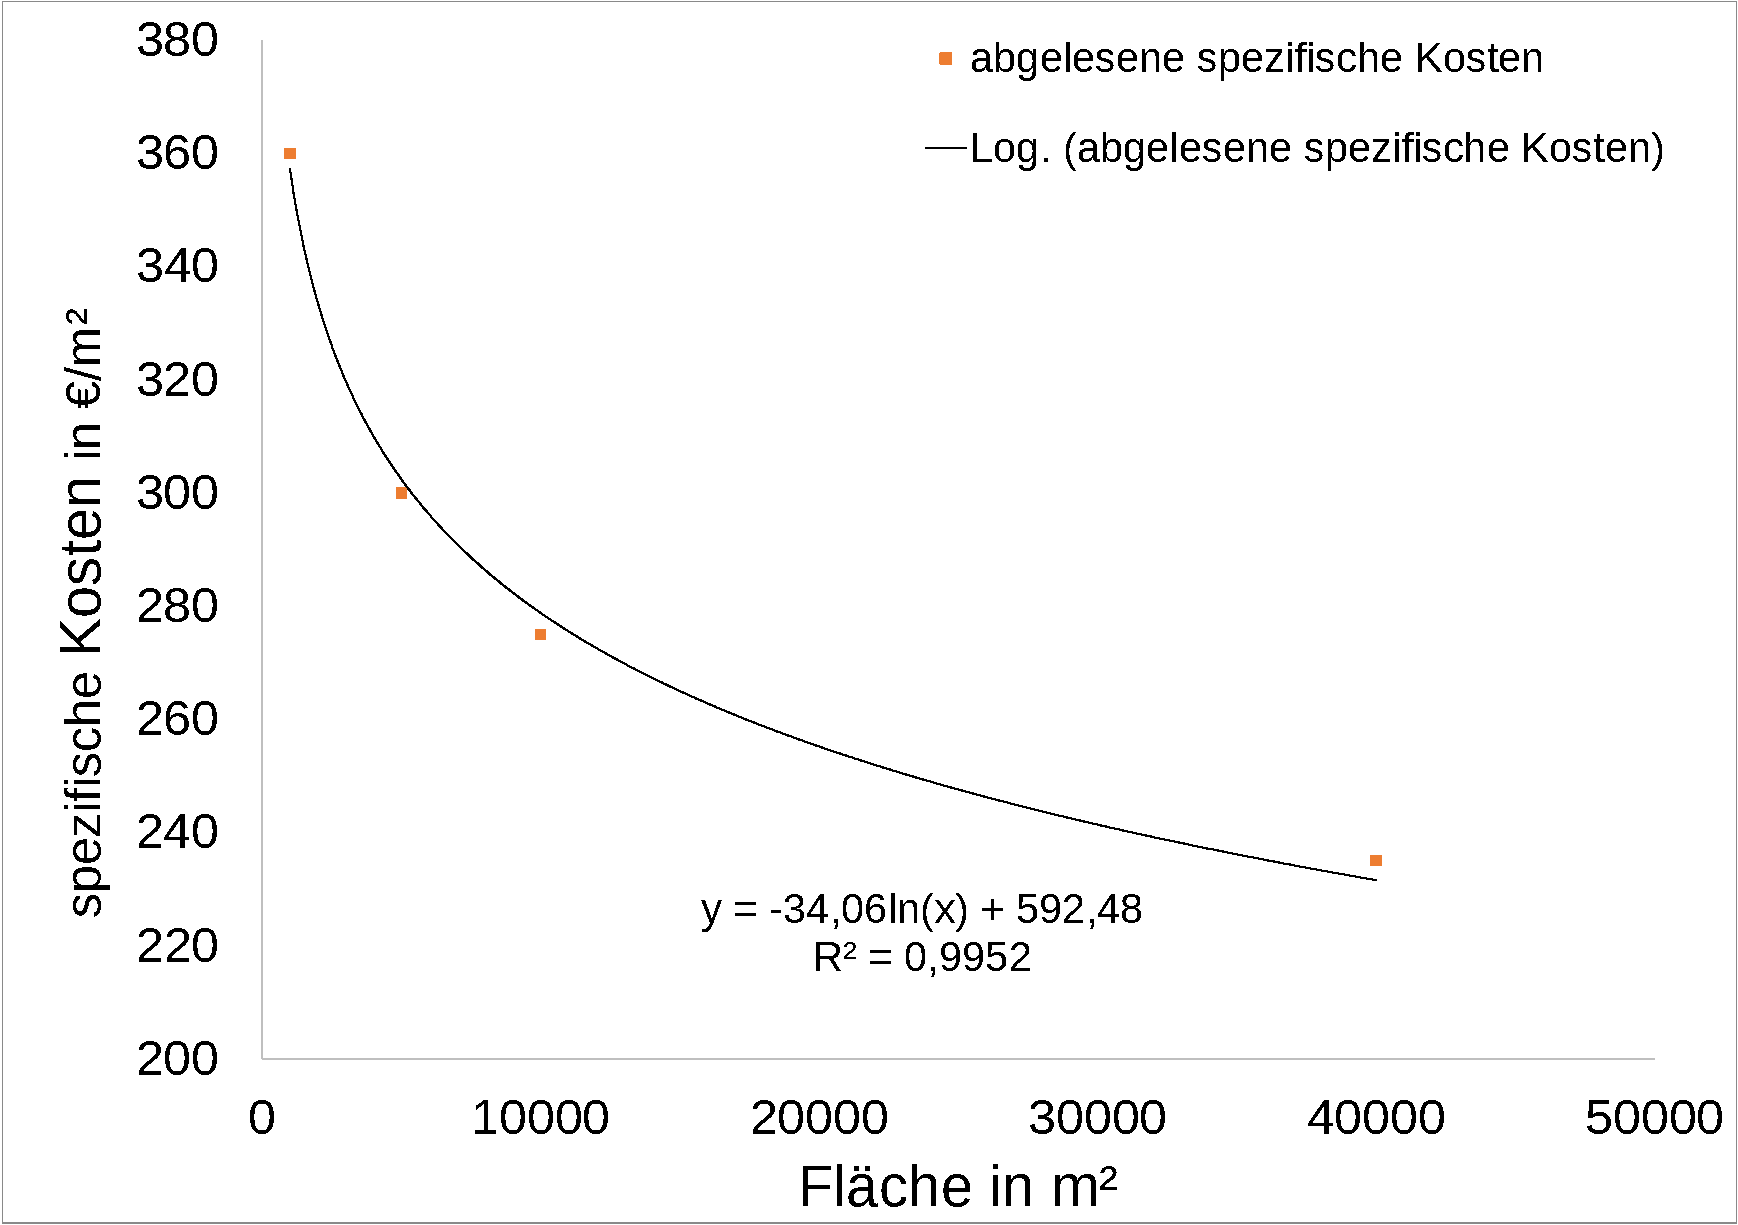
\includegraphics[width=\textwidth]{Kostendegression_Flach-cropped.pdf}
			\subcaption{Flachkollektoren}
		\end{subfigure}
		\begin{subfigure}[b]{0.49\textwidth}
			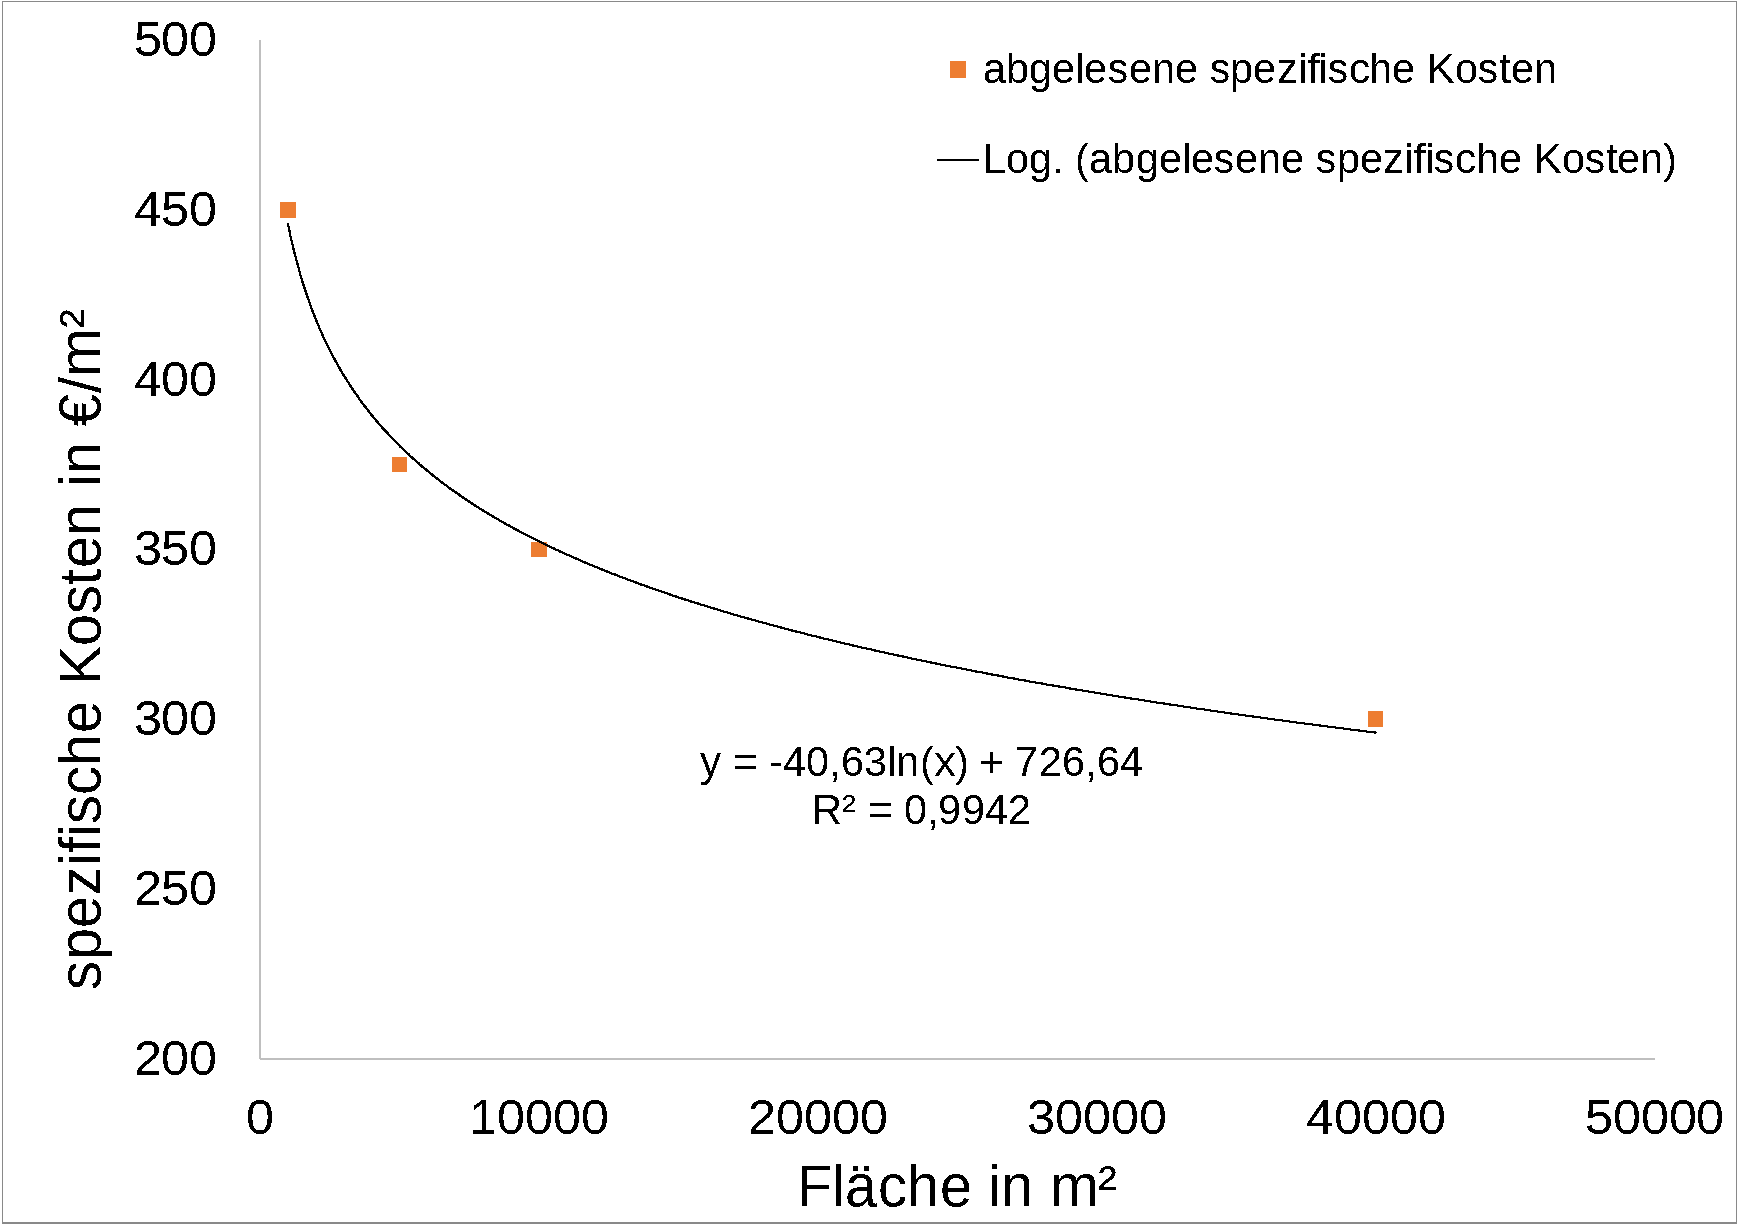
\includegraphics[width=\textwidth]{Kostendegression_Vakuum-cropped.pdf}
			\subcaption{Vakuumröhrenkollektoren}
		\end{subfigure}
		\caption[Darstellung der spezifischen Kosten für Flach- und Vakuumröhrenkollektoren]{Darstellung der spezifischen Kosten für Flach- und Vakuumröhrenkollektoren bei variierender Anlagengröße für vier ausgewählte Anlagengrößen nach \citet{Waermenetz40} sowie die Darstellung der daraus ermittelten logarithmischen Trendlinie}
		\label{fig: Kostendegression Solar}
	\end{figure}

\section{Optimierungsverfahren}\label{section: Optimierungsverfahren}
Ein stetig steigender Anteil volatiler erneuerbarer Energien an der Energieversorgung macht die Vorhersage zu erwartender Erlöse eines Energiesystems zunehmend schwierig. Betriebs- und Einsatzoptimierungen bieten eine Möglichkeit, um einen ökonomisch oder ökologisch optimalen Einsatz des Energiesystems vorherzusagen. So können Aussagen über die Wirtschaftlichkeit geplanter Anlagen getroffen und verschiedene Investitionsmöglichkeiten miteinander verglichen werden. 

In der Energietechnik haben sich lineare und gemischt-ganzzahlige Optimierungsverfahren durchgesetzt, da bei der Optimierung von Energiesystemen häufig ein ganzes Jahr als betrachteter Zeitraum verwendet wird und lange Zeitreihen zu einem überproportional steigenden Rechenaufwand führen. Lineare Probleme sind schneller zu lösen als dynamische und liefern hinreichend genaue Ergebnisse. Somit stellt die lineare Optimierung einen guten Kompromiss zwischen Rechenaufwand und Genauigkeit dar. \cite{GABRIELLI2018408}

Obwohl im Rahmen dieser Arbeit die Software \textit{Solph} genutzt worden ist (vgl. Kapitel \ref{section: Solph}), welche über die Verschaltung von vorgefertigten Komponenten automatisch die mathematische Beschreibung des Problems übernimmt, sollen die folgenden Abschnitte kurz die grundsätzliche Funktionsweise und mathematische Beschreibung der linearen und gemischt-ganzzahligen Optimierung zeigen.  

\subsection{Lineare Optimierung}
Bei der linearen Optimierung (\ac{LP}) wird das Maximum oder Minimum einer linearen Funktion, der sogenannten Zielfunktion $Z$ (objective function) gesucht. Das Überführen eines Minimierungsproblems in ein Maximierungsproblem und umgekehrt kann über die Multiplikation der Zielfunktion mit dem Faktor $(-1)$ erreicht werden. Allgemein kann die Zielfunktion wie in Gleichung \ref{equation: Zielfunktion} dargestellt werden \cite{Stoecker2008}.
	\begin{equation}\label{equation: Zielfunktion}
		\text{\textbf{min }}  Z(x_1, x_2, ..., x_n) = c_1x_1 + c_2x_2 + ... + c_nx_n = \sum_{j=1}^{n}c_jx_j
	\end{equation}
Die Zielfunktion wird aus den Strukturvariablen $x_j$ und den Strukturkonstanten $c_j$ gebildet. Die Strukturvariablen sind im Rahmen dieser Arbeit zum Beispiel die abgegebenen und aufgenommenen Wärmeströme der entsprechenden Komponenten, wohingegen die Strukturkonstanten die spezifischen Kosten der Strukturvariablen darstellen.

Die Optimierung der Zielfunktion erfolgt unter Berücksichtigung von Nebenbedingungen (Constraints). Neben den Nichtnegativitätsbedingungen, die fordern, dass die Strukturvariablen keine negativen Werte annehmen dürfen $x_j \geq 0$, werden Nebenbedingungen genutzt, um das Betriebsverhalten der Anlagen darzustellen. Allgemein werden die Nebenbedingungen als Linearkombination der Strukturvariablen dargestellt. In Gleichung \ref{equation: Nebenbedingungen} wird dies entsprechend veranschaulicht \cite{Vanderbei2014}.
	\begin{equation}\label{equation: Nebenbedingungen}
		a_1x_1 + a_2x_2 + ... +  a_nx_n \begin{Bmatrix}\geq\\=\\\leq\end{Bmatrix} b
	\end{equation} 
Ungleichungen und Gleichungen können immer ineinander überführt werden. Auf diese Weise ist das System auf eine gewünschte Form zu bringen. Können nicht alle Nebenbedingungen erfüllt werden, ist das Problem nicht lösbar (infeasible). Dementsprechend ist ein \ac{LP}-Problem lösbar (feasible), sofern alle Nebenbedingungen erfüllbar sind.

Das aufgestellte System aus Gleichungen und Ungleichungen kann unter Verwendung verschiedener Verfahren gelöst werden. Das wohl bekannteste Verfahren ist die Simplex-Methode, bei der ausgehend von einer Lösung ($x_1, x_2, ..., x_n$) iterativ nach einer anderen Lösung ($x_1^{'}, x_2^{'}, ..., x_n^{'}$) gesucht wird, die einen geringeren Wert der Zielfunktion aufweist. Dies wird so lange wiederholt, bis kein besseres Ergebnis mehr gefunden werden kann \cite{Vanderbei2014}. 

\subsection{Gemischt-ganzzahlig lineare Optimierung}
Bei der gemischt-ganzzahlig linearen Optimierung (\ac{MILP}) sind, im Gegensatz zur einfachen linearen Optimierung, alle oder wenigstens einige Variablen ganzzahlig bzw. diskret \cite{Kallrath2013}. Dies kann bei Energiesystemen zum Beispiel für Erzeugungsanlagen der Fall sein, die entweder im ein- oder ausgeschalteten Zustand sind. In diesem Fall würden die Variablen den Wert Eins oder Null annehmen. Die Verwendung des \ac{MILP}-Verfahrens erlaubt eine genauere Abbildung des Energiesystems, ist jedoch mit einem erhöhten Rechenaufwand verbunden.

Nach \citet{Kallrath2013} können aufgrund effizienterer Verfahren und besserer Solver auch komplexe und umfangreiche \ac{MILP}-Probleme in kurzer Zeit gelöst werden. Dies ist ein Grund, wieso \ac{MILP} ein Standardverfahren bei der Betriebsoptimierung in der Energietechnik ist. So wurde diese Methode unter anderem von \citet{HAIKARAINEN2014211}, \citet{GABRIELLI2018408} und \citet{MORVAJ2016619} zur Untersuchung von Solarthermie in Wärmenetzen genutzt. Im Rahmen dieser Arbeit wird ebenfalls die gemischt-ganzzahlige Optimierung verwendet.

